\subsection{Panel estad�stico de consumo de electricidad por sector}

En la figura ~\ref{fig:EstadisticaDeConsumoDeElectricidadPorSector1990-2014} se presenta un gr�fico con el consumo de energ�a hist�rica, que abarca desde el a�o 1990 hasta 2014. Estos datos est�n clasificados por los siguientes criterios de la ANDE: Alumbrado P�blico, Comercial, Exportaci�n, Gubernamental, Industrial y Residencial. En este gr�fico se puede apreciar que el mayor consumo de energ�a se encuentra en el sector Residencial. Sin embargo, los valores de Exportaci�n de energ�a fue disminuyendo durante el tiempo. Esto tiene sentido debido a que ambos valores son inversamente proporcionales, esto es, cuando el consumo nacional se incrementa, se hace un mayor uso de energ�a en el pa�s, por lo tanto disminuye la energ�a disponible para exportaci�n.

\textsc{\begin{figure}[H]
	\centering
	\caption{Estad�stica de consumo de electricidad por sector(1990-2014)}
	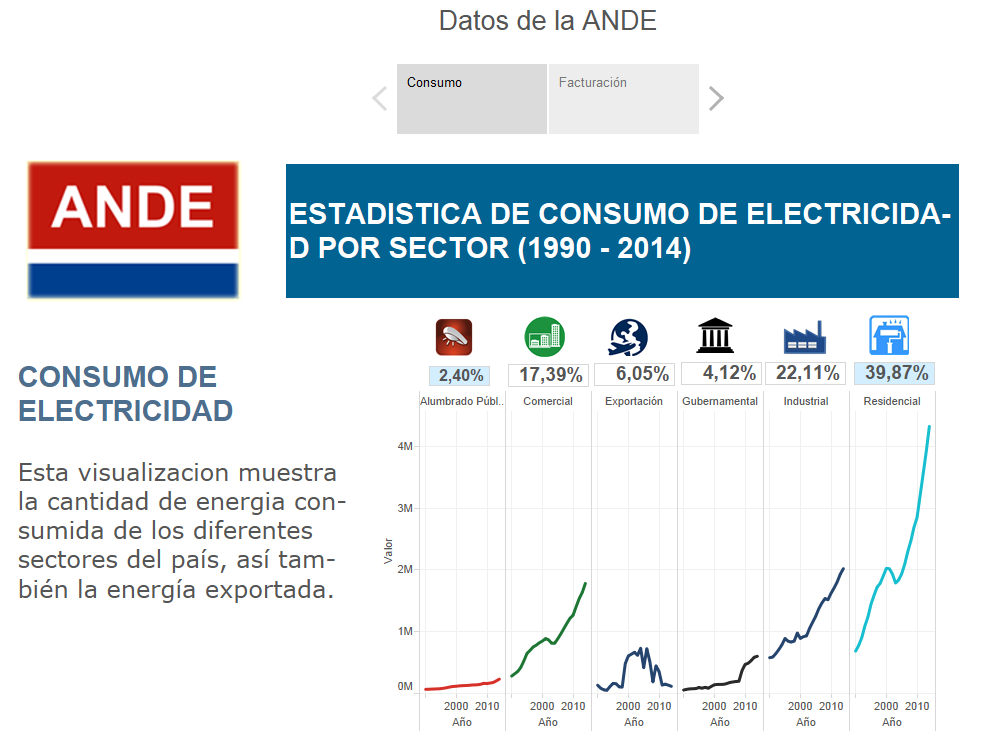
\includegraphics[width=\linewidth]{imagenes/EstadisticaDeConsumoDeElectricidadPorSector1990-2014}
	\caption*{Fuente: Elaboraci�n propia.}
	\label{fig:EstadisticaDeConsumoDeElectricidadPorSector1990-2014}
\end{figure}}

\noindent
La Figura ~\ref{fig:ImporteFacturadoPorAnoYSector1990-2014} presenta las informaciones de facturaci�n tambi�n clasificados por sector, con el recurso de filtros por a�o. Es importante destacar un factor resaltante: aunque energ�a exportada disminuy�, el valor facturado por energ�a vendida al exterior aument�. Es probable que esto se haya debido al aumento de la tarifa de energ�a vendida, lo cual beneficia al pa�s.

\textsc{\begin{figure}[H]
	\centering
	\caption{Importe facturado por a�o y sector(1990-2014)}
	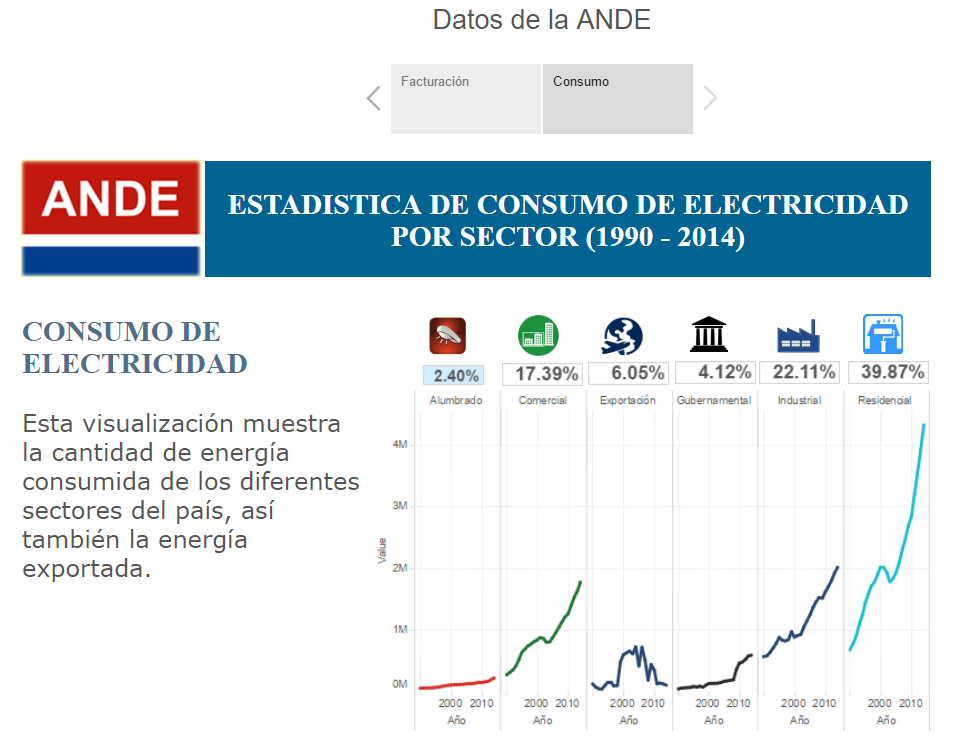
\includegraphics[width=\linewidth]{imagenes/ImporteFacturadoPorAnoYSector1990-2014}
	\caption*{Fuente: Elaboraci�n propia.}
	\label{fig:ImporteFacturadoPorAnoYSector1990-2014}
\end{figure}}
